\documentclass[12pt]{article}

\usepackage{enumitem}
\usepackage{hyperref}
\usepackage{amsthm}
\usepackage{tikz}
\usepackage{amsmath}
\usepackage{color}

\theoremstyle{definition}
\newtheorem{definition}{Definition}[section]

\theoremstyle{definition}
\newtheorem{exmp}{Example}[section]

\newtheorem{theorem}{Theorem}

\title{C\&O URA Spring 2017}
\author{Zach Dockstader}

\begin{document}
\maketitle

\section{Areas of Focus}

\begin{enumerate}[label*=\arabic*.]
	\item Inertia Bounds
	\begin{enumerate}[label*=\arabic*.]
	\item Algorithm to Find Graphs Lacking a 		Tight Interia Bound
	\end{enumerate}
\end{enumerate}


\section{Inertia Bounds}

\subsection{Introduction on Inertia Bounds}
\theoremstyle{definition}
\begin{definition}{Independent Set}
An independent set is a set of vertices belonging to a graph in which no two vertices are adjacent.
\end{definition}
\begin{exmp}
Consider the following graph:\\
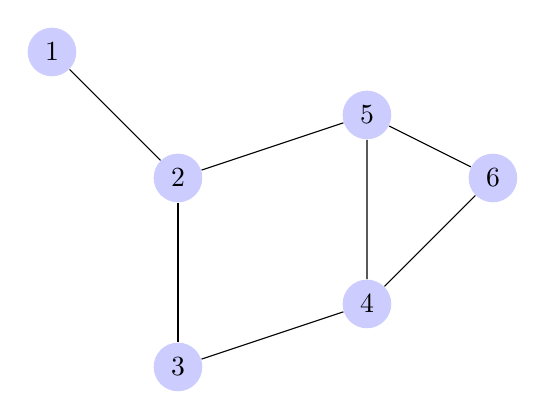
\begin{tikzpicture}
[scale=.8,every node/.style={circle,fill=blue!20}]
\node (n1) at (1,10) {1};
\node (n2) at (3,8) {2};
\node (n3) at (3,5) {3};
\node (n4) at (6,6) {4};
\node (n5) at (6,9) {5};
\node (n6) at (8,8) {6};
\foreach \from/\to in {n1/n2,n2/n3,n2/n5,n3/n4,n5/n4,n5/n6,n4/n6}
\draw (\from) -- (\to);
\end{tikzpicture}

An example of an independent set in this graph is:\\
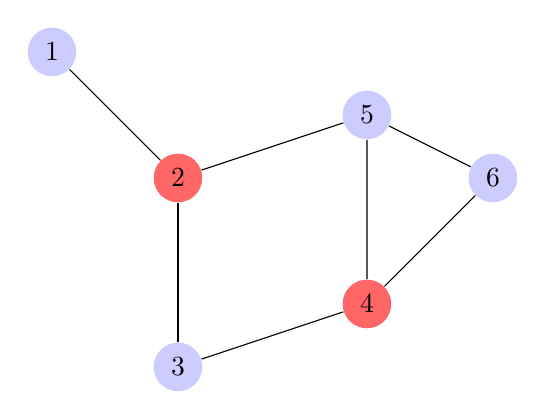
\begin{tikzpicture}
[scale=.8,every node/.style={circle,fill=blue!20}]
\node (n1) at (1,10) {1};
\node[fill=red!60] (n2) at (3,8) {2};
\node (n3) at (3,5) {3};
\node[fill=red!60] (n4) at (6,6) {4};
\node (n5) at (6,9) {5};
\node (n6) at (8,8) {6};
\foreach \from/\to in {n1/n2,n2/n3,n2/n5,n3/n4,n5/n4,n5/n6,n4/n6}
\draw (\from) -- (\to);
\end{tikzpicture}

However, often the independent set we are most interested in finding is the largest one:\\
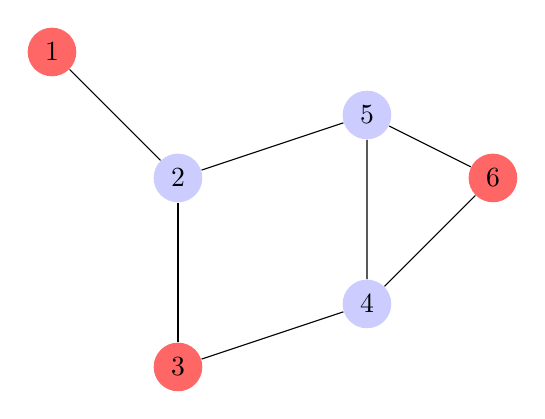
\begin{tikzpicture}
[scale=.8,every node/.style={circle,fill=blue!20}]
\node[fill=red!60] (n1) at (1,10) {1};
\node (n2) at (3,8) {2};
\node[fill=red!60] (n3) at (3,5) {3};
\node (n4) at (6,6) {4};
\node (n5) at (6,9) {5};
\node[fill=red!60] (n6) at (8,8) {6};
\foreach \from/\to in {n1/n2,n2/n3,n2/n5,n3/n4,n5/n4,n5/n6,n4/n6}
\draw (\from) -- (\to);
\end{tikzpicture}
\end{exmp}
\begin{definition}{Independence Number}
The independence number of a graph G, denoted $\alpha$(G), is the size of the largest independent set of G.
\end{definition}

\begin{definition}{Weight Matrix}
The weight matrix of a graph G, is a matrix defined by:

\begin{equation}
    W_{i,j} = 
    \begin{cases}
        1 & \mbox{if $v_i$ and $v_j$ are adjacent} \\
        0 & \mbox{otherwise}
    \end{cases}
\end{equation}
with $v_i$ a vertice of G.

\end{definition}

For any graph G, there exists a bound on $\alpha$(G), known as the Cvetkovi\'c bound (also referred to as the Interia Bound). This bound provides a relationship between $\alpha$(G) and the number of positive, negative, and zero eigenvalues of the weight matrix, W, associated with G. The Cvetkovi\'c bound of G, is:

\begin{equation}
\alpha(G) \leq min\{|G| - n_+(W),|G|-n_-(W)\}
\end{equation}

Where $n_+(W)$ and $n_-(W)$ denote the number of positive and negative eigenvalues of W, respectively.

To prove this, we first need to introduce the Eigenvalue Interlacing Theorem:

\begin{theorem}{Eigenvalue Interlacing Theorem}
Let A be an $n\times n$ real symmetric matrix with eigenvalues $\lambda_1 \geq \lambda_2 \geq \ldots \geq \lambda_n$ and let C be a $k\times k$ principal submatrix of A with eigenvalues $\tau_1 \geq \tau_2 \geq \ldots \geq \tau_k$. Then $\lambda_i \geq \tau_i$ for all i $\in \{1,\ldots ,k\}$. *****(CITE FROM JOHNS PAPER)******
\end{theorem}

\begin{definition}{Principal Submatrix}
The principal submatrix of an $n\times n$ matrix A is the submatrix obtained where if $row_i$ is excluded in the submatrix, then $column_i$ is excluded as well. Note that all principal submatrices of a weight matrix W, correspond to an induced subgraph in the graph represented by W.
\end{definition}

\begin{exmp}
The following is an example of a principal submatrix in relation to graph theory.

Consider the following graph:

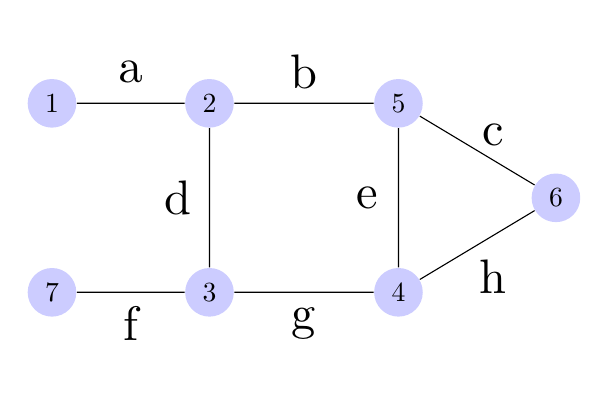
\begin{tikzpicture}
[scale=.8,every node/.style={circle,fill=blue!20}]
\node[scale=1.75,fill=white] (a) at (2.75,9.5) {a};
\node[scale=1.75,fill=white] (b) at (5.5,9.5) {b};
\node[scale=1.75,fill=white] (c) at (8.5,8.5) {c};
\node[scale=1.75,fill=white] (d) at (3.5,7.5) {d};
\node[scale=1.75,fill=white] (e) at (6.5,7.5) {e};
\node[scale=1.75,fill=white] (f) at (2.75,5.5) {f};
\node[scale=1.75,fill=white] (g) at (5.5,5.5) {g};
\node[scale=1.75,fill=white] (h) at (8.5,6.25) {h};
\node (n1) at (1.5,9) {1};
\node (n2) at (4,9) {2};
\node (n3) at (4,6) {3};
\node (n4) at (7,6) {4};
\node (n5) at (7,9) {5};
\node (n6) at (9.5,7.5) {6};
\node (n7) at (1.5,6) {7};
\foreach \from/\to in {n1/n2,n2/n3,n2/n5,n3/n4,n5/n4,n5/n6,n4/n6,n3/n7}
\draw (\from) -- (\to);
\end{tikzpicture}

and corresponding weight matrix:

$
\begin{bmatrix}
0 & a & 0 & 0 & 0 & 0 & 0 \\
a & 0 & d & 0 & b & 0 & 0 \\
0 & d & 0 & g & 0 & 0 & f \\
0 & 0 & g & 0 & e & h & 0 \\
0 & b & 0 & e & 0 & c & 0 \\
0 & 0 & 0 & h & c & 0 & 0 \\
0 & 0 & f & 0 & 0 & 0 & 0 \\
\end{bmatrix}
$
\\
We can see the following principal submatrix and corresponding induced subgraph:

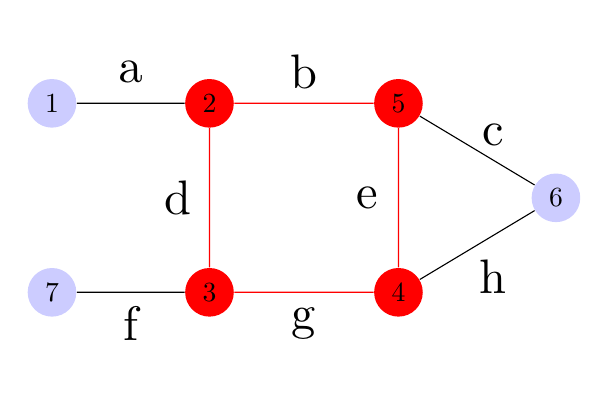
\begin{tikzpicture}
[scale=.8,every node/.style={circle,fill=blue!20}]
\node[scale=1.75,fill=white] (a) at (2.75,9.5) {a};
\node[scale=1.75,fill=white] (b) at (5.5,9.5) {b};
\node[scale=1.75,fill=white] (c) at (8.5,8.5) {c};
\node[scale=1.75,fill=white] (d) at (3.5,7.5) {d};
\node[scale=1.75,fill=white] (e) at (6.5,7.5) {e};
\node[scale=1.75,fill=white] (f) at (2.75,5.5) {f};
\node[scale=1.75,fill=white] (g) at (5.5,5.5) {g};
\node[scale=1.75,fill=white] (h) at (8.5,6.25) {h};
\node (n1) at (1.5,9) {1};
\node[fill=red] (n2) at (4,9) {2};
\node[fill=red] (n3) at (4,6) {3};
\node[fill=red] (n4) at (7,6) {4};
\node[fill=red] (n5) at (7,9) {5};
\node (n6) at (9.5,7.5) {6};
\node (n7) at (1.5,6) {7};
\foreach \from/\to in {n1/n2,n5/n6,n4/n6,n3/n7}
\draw (\from) -- (\to);
\draw[red](n2) -- (n5);
\draw[red](n2) -- (n3);
\draw[red](n3) -- (n4);
\draw[red](n4) -- (n5);
\end{tikzpicture}

$
\begin{bmatrix}
0 & a & 0 & 0 & 0 & 0 & 0 \\
a & \color{red}0 & \color{red}d & \color{red}0 & \color{red}b & 0 & 0 \\
0 & \color{red}d & \color{red}0 & \color{red}g & \color{red}0 & 0 & f \\
0 & \color{red}0 & \color{red}g & \color{red}0 & \color{red}e & h & 0 \\
0 & \color{red}b & \color{red}0 & \color{red}e & \color{red}0 & c & 0 \\
0 & 0 & 0 & h & c & 0 & 0 \\
0 & 0 & f & 0 & 0 & 0 & 0 \\
\end{bmatrix}
$

As well, we see the following principal submatrix of an independent set of the graph:

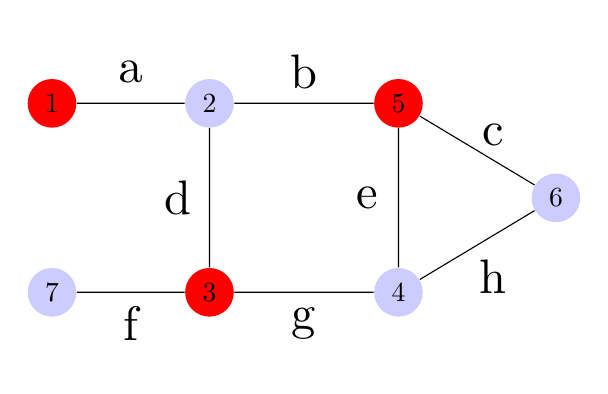
\begin{tikzpicture}
[scale=.8,every node/.style={circle,fill=blue!20}]
\node[scale=1.75,fill=white] (a) at (2.75,9.5) {a};
\node[scale=1.75,fill=white] (b) at (5.5,9.5) {b};
\node[scale=1.75,fill=white] (c) at (8.5,8.5) {c};
\node[scale=1.75,fill=white] (d) at (3.5,7.5) {d};
\node[scale=1.75,fill=white] (e) at (6.5,7.5) {e};
\node[scale=1.75,fill=white] (f) at (2.75,5.5) {f};
\node[scale=1.75,fill=white] (g) at (5.5,5.5) {g};
\node[scale=1.75,fill=white] (h) at (8.5,6.25) {h};
\node[fill=red] (n1) at (1.5,9) {1};
\node (n2) at (4,9) {2};
\node[fill=red] (n3) at (4,6) {3};
\node (n4) at (7,6) {4};
\node[fill=red] (n5) at (7,9) {5};
\node (n6) at (9.5,7.5) {6};
\node (n7) at (1.5,6) {7};
\foreach \from/\to in {n1/n2,n2/n3,n2/n5,n3/n4,n5/n4,n5/n6,n4/n6,n3/n7}
\draw (\from) -- (\to);
\end{tikzpicture}

$
\begin{bmatrix}
\color{red}0 & a & \color{red}0 & 0 & \color{red}0 & 0 & 0 \\
a & 0 & d & 0 & b & 0 & 0 \\
\color{red}0 & d & \color{red}0 & g & \color{red}0 & 0 & f \\
0 & 0 & g & 0 & e & h & 0 \\
\color{red}0 & b & \color{red}0 & e & \color{red}0 & c & 0 \\
0 & 0 & 0 & h & c & 0 & 0 \\
0 & 0 & f & 0 & 0 & 0 & 0 \\
\end{bmatrix}
$

\end{exmp}

Now to prove the Cvetkovi\'c Bound:

\begin{theorem}{Cvetkovi\'c Bound}
Let G be a graph on n vertices, and W be the weight matrix of G. Then the following inequality holds:
\begin{equation}
\alpha(G) \leq min\{|G| - n_+(W),|G|-n_-(W)\}
\end{equation}
\end{theorem}

\begin{proof}
Let H be the subgraph of G formed by the vertices in an independent set of size s. Then H is an induced subgraph of G and all eigenvalues of the principal submatrix W(H) are 0 since the principal submatrix will just be a zero matrix. Let $\lambda_i$ denote the ith largest eigenvalue of W and $\tau_i$ denote the ith larest eigenvalue of W(H). Now, by interlacing, we have,
\begin{equation}
\lambda_i \geq \tau_i = 0 \text{ for all i } \in \{1,\ldots ,s\}
\end{equation}

and so 
\begin{equation}
n - n_-(W) = n_+(W) + n_0(W) \geq s
\end{equation}
Also, note that by negating W, the positive eigenvalues become negative eigenvalues and vice versa. Thus,
\begin{equation}
n - n_+(W) = n - n_-(-W),
\end{equation}
However, the principal submatrix corresponding to H in -W is still the zero matrix and thus has all zero eigenvalues. Thus, by interlacing, we get a similar result as above, 
\begin{equation}
n - n_+(W) = n - n_-(-W) = n_+(-W) + n_0(-W) \geq s
\end{equation}

Therefore, both $n - n_+(W)$ and $n - n_-(W)$ are greater than or equal to s. Since s is the size of the idependent set, we can see that letting s = $\alpha$(G), we get:

\begin{equation}
\alpha(G) \leq min\{|G| - n_+(W),|G|-n_-(W)\}
\end{equation}

\end{proof}

\end{document}



